\documentclass[11pt,a4paper,dvipdfmx]{jsarticle}
%
\usepackage{amsmath,amssymb,amsthm}
\usepackage{bm}
\usepackage{graphicx}
\usepackage{ascmac}
\usepackage{physics}
%
\setlength{\textwidth}{\fullwidth}
\setlength{\textheight}{39\baselineskip}
\addtolength{\textheight}{\topskip}
\setlength{\voffset}{-0.5in}
\setlength{\headsep}{0.3in}
%
\title{テンプレ}
\author{pj}
\date{\today}
%
\begin{document}
\maketitle
   \section{画像}
   %%%% 図 %%%%
         \begin{figure}[h!]
            \begin{tabular}{cc}
               %---- 最初の図 --------------------------
               \begin{minipage}[t]{0.5\hsize}
                  \centering
                  
\includegraphics[scale=0.5]{./images/cat.jpeg}
                  \caption{cat}
                  \label{fig:cat}
               \end{minipage} 
               %---- 2番目の図 --------------------------
               \begin{minipage}[t]{0.5\hsize}
                  \centering
                  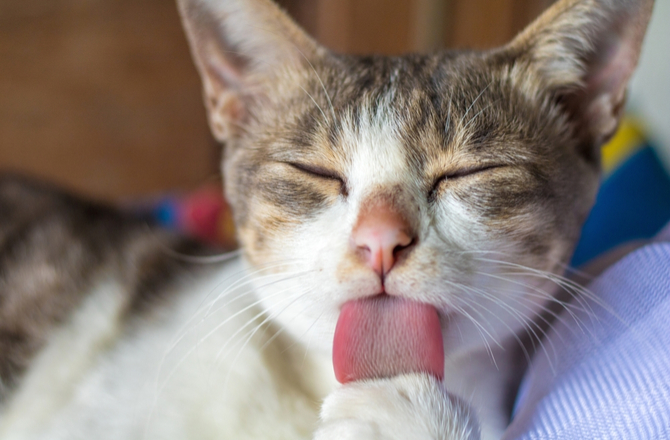
\includegraphics[scale=0.5]{./images/cat2.jpg}
                  \caption{cat}
                  \label{fig:cat2}
               \end{minipage}  \\ 
               %-----------------------------------------
               %---- 最初の図 --------------------------
               \begin{minipage}[t]{0.5\hsize}
                  \centering
                  
\includegraphics[scale=0.5]{./images/doge.jpeg}
                  \caption{doge}
                  \label{fig:doge}
               \end{minipage} 
               %---- 2番目の図 --------------------------
               \begin{minipage}[t]{0.5\hsize}
                  \centering
                  
\includegraphics[scale=0.5]{./images/hari.jpeg}
                  \caption{ハリネズミ}
                  \label{fig:hari}
               \end{minipage} \\
            \end{tabular}
         \end{figure}
   \section{原理}
   \section{原理}
   \section{実験}
   \section{考察}
   \section{結論} 
\end{document}
